% exercise sheet with header on every page for math or close subjects
\documentclass[12pt]{article}
\usepackage[utf8]{inputenc}
\usepackage{latexsym}
\usepackage{multicol}
\usepackage{fancyhdr}
\usepackage{amsfonts}
\usepackage{amsmath}
\usepackage{amssymb}
\usepackage{enumerate}
\usepackage{listings}
\usepackage{graphicx}

% Shortcuts for bb, frak and cal letters
\newcommand{\E}{\mathbb{E}}
\newcommand{\V}{\mathbb{V}}
\renewcommand{\P}{\mathbb{P}}
\newcommand{\N}{\mathbb{N}}
\newcommand{\R}{\mathbb{R}}
\newcommand{\C}{\mathbb{C}}
\newcommand{\Z}{\mathbb{Z}}
\newcommand{\Pfrak}{\mathfrak{P}}
\newcommand{\Pfrac}{\mathfrak{P}}
\newcommand{\Bfrac}{\mathfrak{P}}
\newcommand{\Bfrak}{\mathfrak{B}}
\newcommand{\Fcal}{\mathcal{F}}
\newcommand{\Ycal}{\mathcal{Y}}
\newcommand{\Bcal}{\mathcal{B}}
\newcommand{\Acal}{\mathcal{A}}

% formating
\topmargin -3.5cm
\textheight 22cm
\textwidth 16.0 cm
\oddsidemargin -0.1cm

% Fancy Header on every Page
\pagestyle{fancy}
\lhead{\textbf{Embedded Systems Milestone 1}}
\rhead{Daniel Schäfer (2549458)\\ Rafael Dewes (2548365)\\ Kevin M\"uller (2550062)}
\renewcommand{\headrulewidth}{1.2pt}
\setlength{\headheight}{110pt}

\begin{document}
\pagenumbering{gobble}
\lstset{language=C++}

\section*{Pins - Scout}

\paragraph{Must not be driven in Combination:}
The only Pins that can not be driven simultaniously are the PINS PD4 and PC5. These PINS are used for the SPI Protocol to select either the ADC and RF module as the "receiver" of a message and only one of the chips can be selected using either PIN PD4 OR Pin PC5.

\paragraph{Must be driven in Combination:}
During the entire process of transfering data using SPI, it is obvious that PB4 has to "run" all the time to ensure that Master and Slaves communicate in a  synchronized manner. To achieve this Data is transfered over the lane with the Clockrate given by SCK. Both MOSI and MISO lanes can only be driven when one of the Slave Select Lanes is driven aswell (either PD4 or PC5 in case of scout).

\small
\begin{tabular}{| c || p{30mm} | p{30mm} | p{60mm} |}
  \hline
  \textbf{PIN} & FUNCTION & alternate Functions & NOTES\\
  \hline
  \hline
  \textbf{PB4} & I/O Clock of ADC & SCK of RF module & Synchronisation Clock of Serial Peripheral Interface (Master Slave Connection/SPI).\\
  \hline
  \textbf{PB5} & MOSI lane to ADC & MOSI lane to RF & Master Output, Slave Input lane. The Slave Select lane (PD4/PC5) determines with which of the slaves (either RF module or ADC) the master communicates. This lane is used to communicate to the ADC of which photoresistor data should be read and to communicate information to the RF module.\\
  \hline
  \textbf{PB0} & MISO lane to ADC & MISO lane to RF & Master Input, Slave Output lane. The master receives either the output of the data out lane of the ADC or the output of the MISO lane of the RF.\\
  \hline
  \textbf{PD4} & RF module Chip Select & - & The Slave Select Lane PD4 detimines that the communication over the BUS is with the RF module (and not with the ADC).\\
  \hline
  \textbf{PD7} & RF module Chip Enable & - & Chip Enable Activates RX (used as receiver) or TX Mode (used as transmitter)\\
  \hline
  \textbf{PD2} & RF IRQ & - & Maskable interrupt pin. Active low. Confirms either packet arrival when package loaded into RX FIFO (RX mode) or arrival of ACK (acknowledge) packet (TX mode).\\
  \hline
  \textbf{PB1} & ADC system clock & - & Prescaled Clock source, which allows time for a conversion to happen inside the ADC (I/O Clock must remain low for at least 36 system clock cycles to allow conversion to be completed)\\
  \hline
  \textbf{PC5} & ADC Chip Select & - & The Slave Select Lane PC5 detimines that the communication over the BUS is with the ADC (and not with the RF Module).\\
  \hline
  \textbf{PD0} & Dev Port RX & - & Communication Input of UART Serial Communication (Output atmega328 - Input Dev Port)\\
  \hline
  \textbf{PD1} & Dev Port TX & - & Communication Output of UART Serial Communication (Output Dev Port - Input atmega328)\\
  \hline
\end{tabular}
\normalsize

\vspace{1cm}

\newpage
\section*{Pins - Collector}


\paragraph{Must not be driven in Combination:}
All pins mentioned on the cheatsheet can be driven in combination.

\paragraph{Must be driven in Combination:}
During the entire process of transfering data using SPI, it is obvious that PB0 has to "run" all the time to ensure that Master and Slaves communicate in a  synchronized manner. To achieve this Data is transfered over the lane with the Clockrate given by SCK. Both MOSI and MISO lanes can only be driven when one of the Slave Select Lanes is driven aswell (in the case of collector, this is only PB3 as only one slave is specified on the cheatsheet)\\

\small
\begin{tabular}{| c || p{30mm} | p{30mm} | p{60mm} |}
  \hline
  \textbf{PIN} & FUNCTION & alternate Functions & NOTES\\
  \hline
  \hline
  \textbf{PB0} & RF SCK &  & Serial Clock given by master to synchronize communication over SPI protocol. \\
  \hline
  \textbf{PD5} & RF MOSI &  & Master Output - Slave Input lane used for SPI. This lane will e.g. be used to send package contents to the RF chip.\\
  \hline
  \textbf{PD7} & RF MISO &  & Master Input - Slave Output lane used for SPI. This lane will e.g. be used to receive package contents from the RF chip.\\
  \hline
  \textbf{PB3} & RF chip select &  & This Slave Select Lane detimines that the communication over the BUS is with the RF module\\
  \hline
  \textbf{PC7} & RF chip enable &  & Chip Enable Activates RX (used as receiver) or TX Mode (used as transmitter) \\
  \hline
  \textbf{PD2} & RF IRQ & Dev Port RX & Maskable interrupt pin. Active low. Confirms either packet arrival when package loaded into RX FIFO (RX mode) or arrival of ACK (acknowledge) packet (TX mode). Additionally this lane is the communication Input of UART Serial Communication (Output atmega32u4 - Input Dev Port) \\
  \hline
  \textbf{PD3} & Dev Port TX &  & Communication Output of UART Serial Communication (Output Dev Port - Input atmega32u4) \\
  \hline
\end{tabular}
\normalsize

\newpage
\section*{Interrupts}
3pi/Scout(ATmega 328): \\
\begin{itemize}
\item Finding a location where the photo sensor readings surpass 200 (external)
\item Check for timer $> 5$ minutes (internal)
\end{itemize}
Zumo/Collector(ATmega 32u4): \\
\begin{itemize}
\item Check if communication by Scout $\neq -1$ (external)
\end{itemize} 

\flushleft
\textit{How does the interrupt service routine handle the interrupt? Which pins are affected?} \\

3pi/Scout(ATmega 328): \\
\begin{itemize}
\item Finding a location: INT0, 0x0002
The interrupt is executed asynchronously 
\item Check for timer: TIMER2 COMPA, 0x000E 
\end{itemize}
Zumo/Collector(ATmega 32u4): \\
\begin{itemize}
\item Check Scout communication: INT0, \$0006
\end{itemize}

\textit{Which conditions should an interrupt concerning the communication with the expansion board occur?} \\
\textit{Is the interrupt triggered by an external or internal source?} \\


\newpage
\section*{Hybrid Automata}
\subsection* {Scout}
The scout has two modes of operation: Moving in the dark (areas with photo sensor readings $\leq 200$) and light areas (areas with photo sensor readings $> 200$). The input sensor readings are in the variable photoSignal. In both states, position and angles are modelled as derivates calculated from the left and right angular wheel velocities u\textsubscript{l} and u\textsubscript{r}. For simplicity, we modelled the wheels in a way that they can either turn forward or backward with constant speed of 1. We also introduced continuous variables for the harvesting positions which are only updated in the state MoveInLight. Before that, they remain at $-1$. Those variables as well as the angular wheel velocities are also the output variables. The self-loop in MoveInLight updates the variable bestP with the best photo sensor reading so far. From the exercise we were not sure whether this best value should only include values $> 200$ or all values. If we would want all values we would have to add such a self-loop in the MoveInDark state. Another continuous variable clock keeps track of the time and triggers a transition to state Done after 300 seconds where the best harvesting position read so far will be output.\\
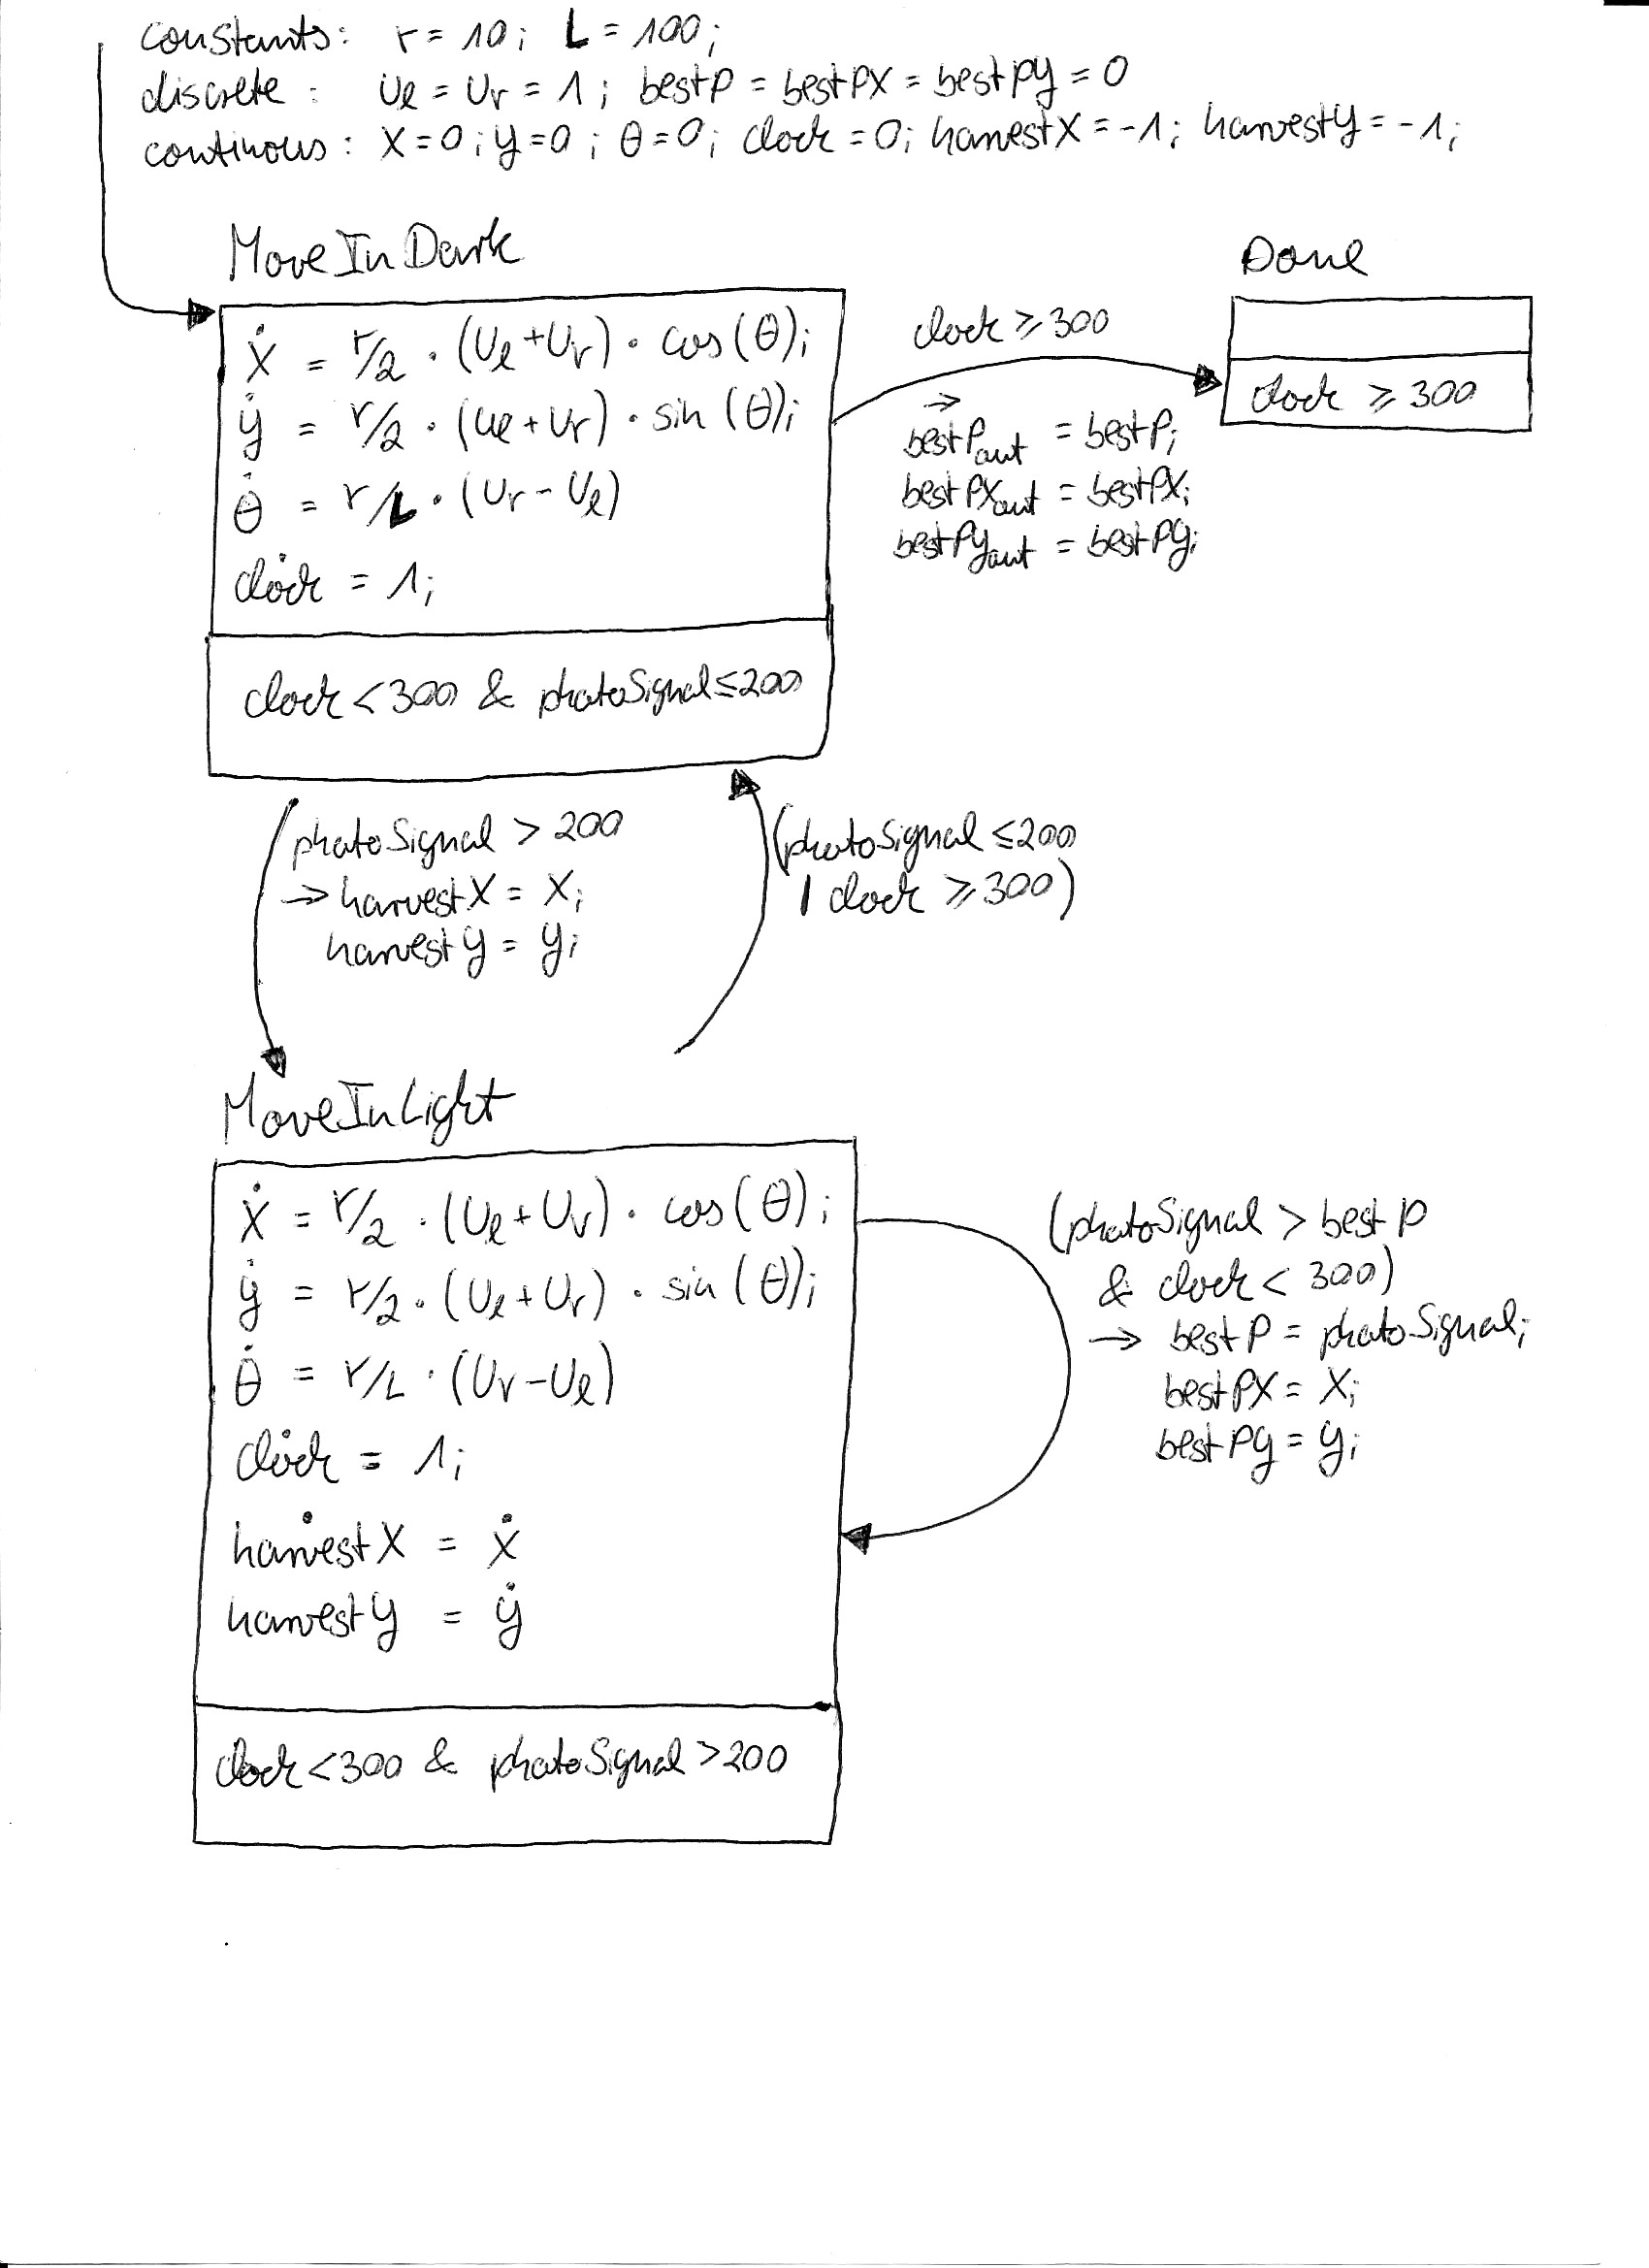
\includegraphics[scale = 0.8]{pictures/hybrid_automata_scout}

\subsection* {Collector}
The collector has two main states: Annoy and Harvest. Input variables are harvestX and harvestY which it gets from the scout and pLeft, pFront and pRight which are the left, front and right proximity sensor readings. In the initial state Annoy, the collector drives forward and turns left or right when the proximity sensors at the sides indicate a nearby object. This is achieved by inverting the angular wheel velocitys, e.g. in order to turn left, we flip u\textsubscript{l} from 1 to -1. Just as for the scout, u\textsubscript{l} and u\textsubscript{r} are our motor control output signals. In the turning state we only have to update $\Theta$ because the robot is not moving forward but only rotating at the same position. Once a harvest signal is received by the scout, the robot transitions to the Harvest state. There, it computes the angle to which it has to turn in order to point to the harvesting position. The function \verb!getAngle()! calculates the required angle:
\begin{lstlisting}
getAngle(x, y, harvestX, harvestY) {
    vec = (harvestY- y, harvestX - x);
    angle = arctan(vec.y / vec.x);
    if (vec.x < 0) 
        angle += 180;
    if (angle > 180) 
        angle = -360 + angle;
    if (angle < -180) 
        angle = 360 - angle;
    return angle;
}
\end{lstlisting}
The robot compares this angle with its current angle $\Theta$  and transitions into either TurnLeft or TurnRight and turns until it points straight at the harvesting position. It then transitions back into the Harvest state where it moves forward towards the harvesting position. Once there, it stops. To ensure that the system does not transition back to Annoy once it has been in Harvest, we introduced the variable a that ensures that states TurnLeft and TurnRight can only transition to the states that transitioned to them and, in particular, not from Harvest to Annoy or vice versa.\\
Note that the turning functionality as we have modelled it for the collector can work in the same way for the scout. For simplicity we have omitted it in the above automaton because given the assumption from the exercise that we have an infinitely large map with no sensible boundaries it does note make a difference whether the scout makes turns or only keeps driving forward. We have also modelled both automata in Stateflow where we let the scout make turns based on the current clock value.\\
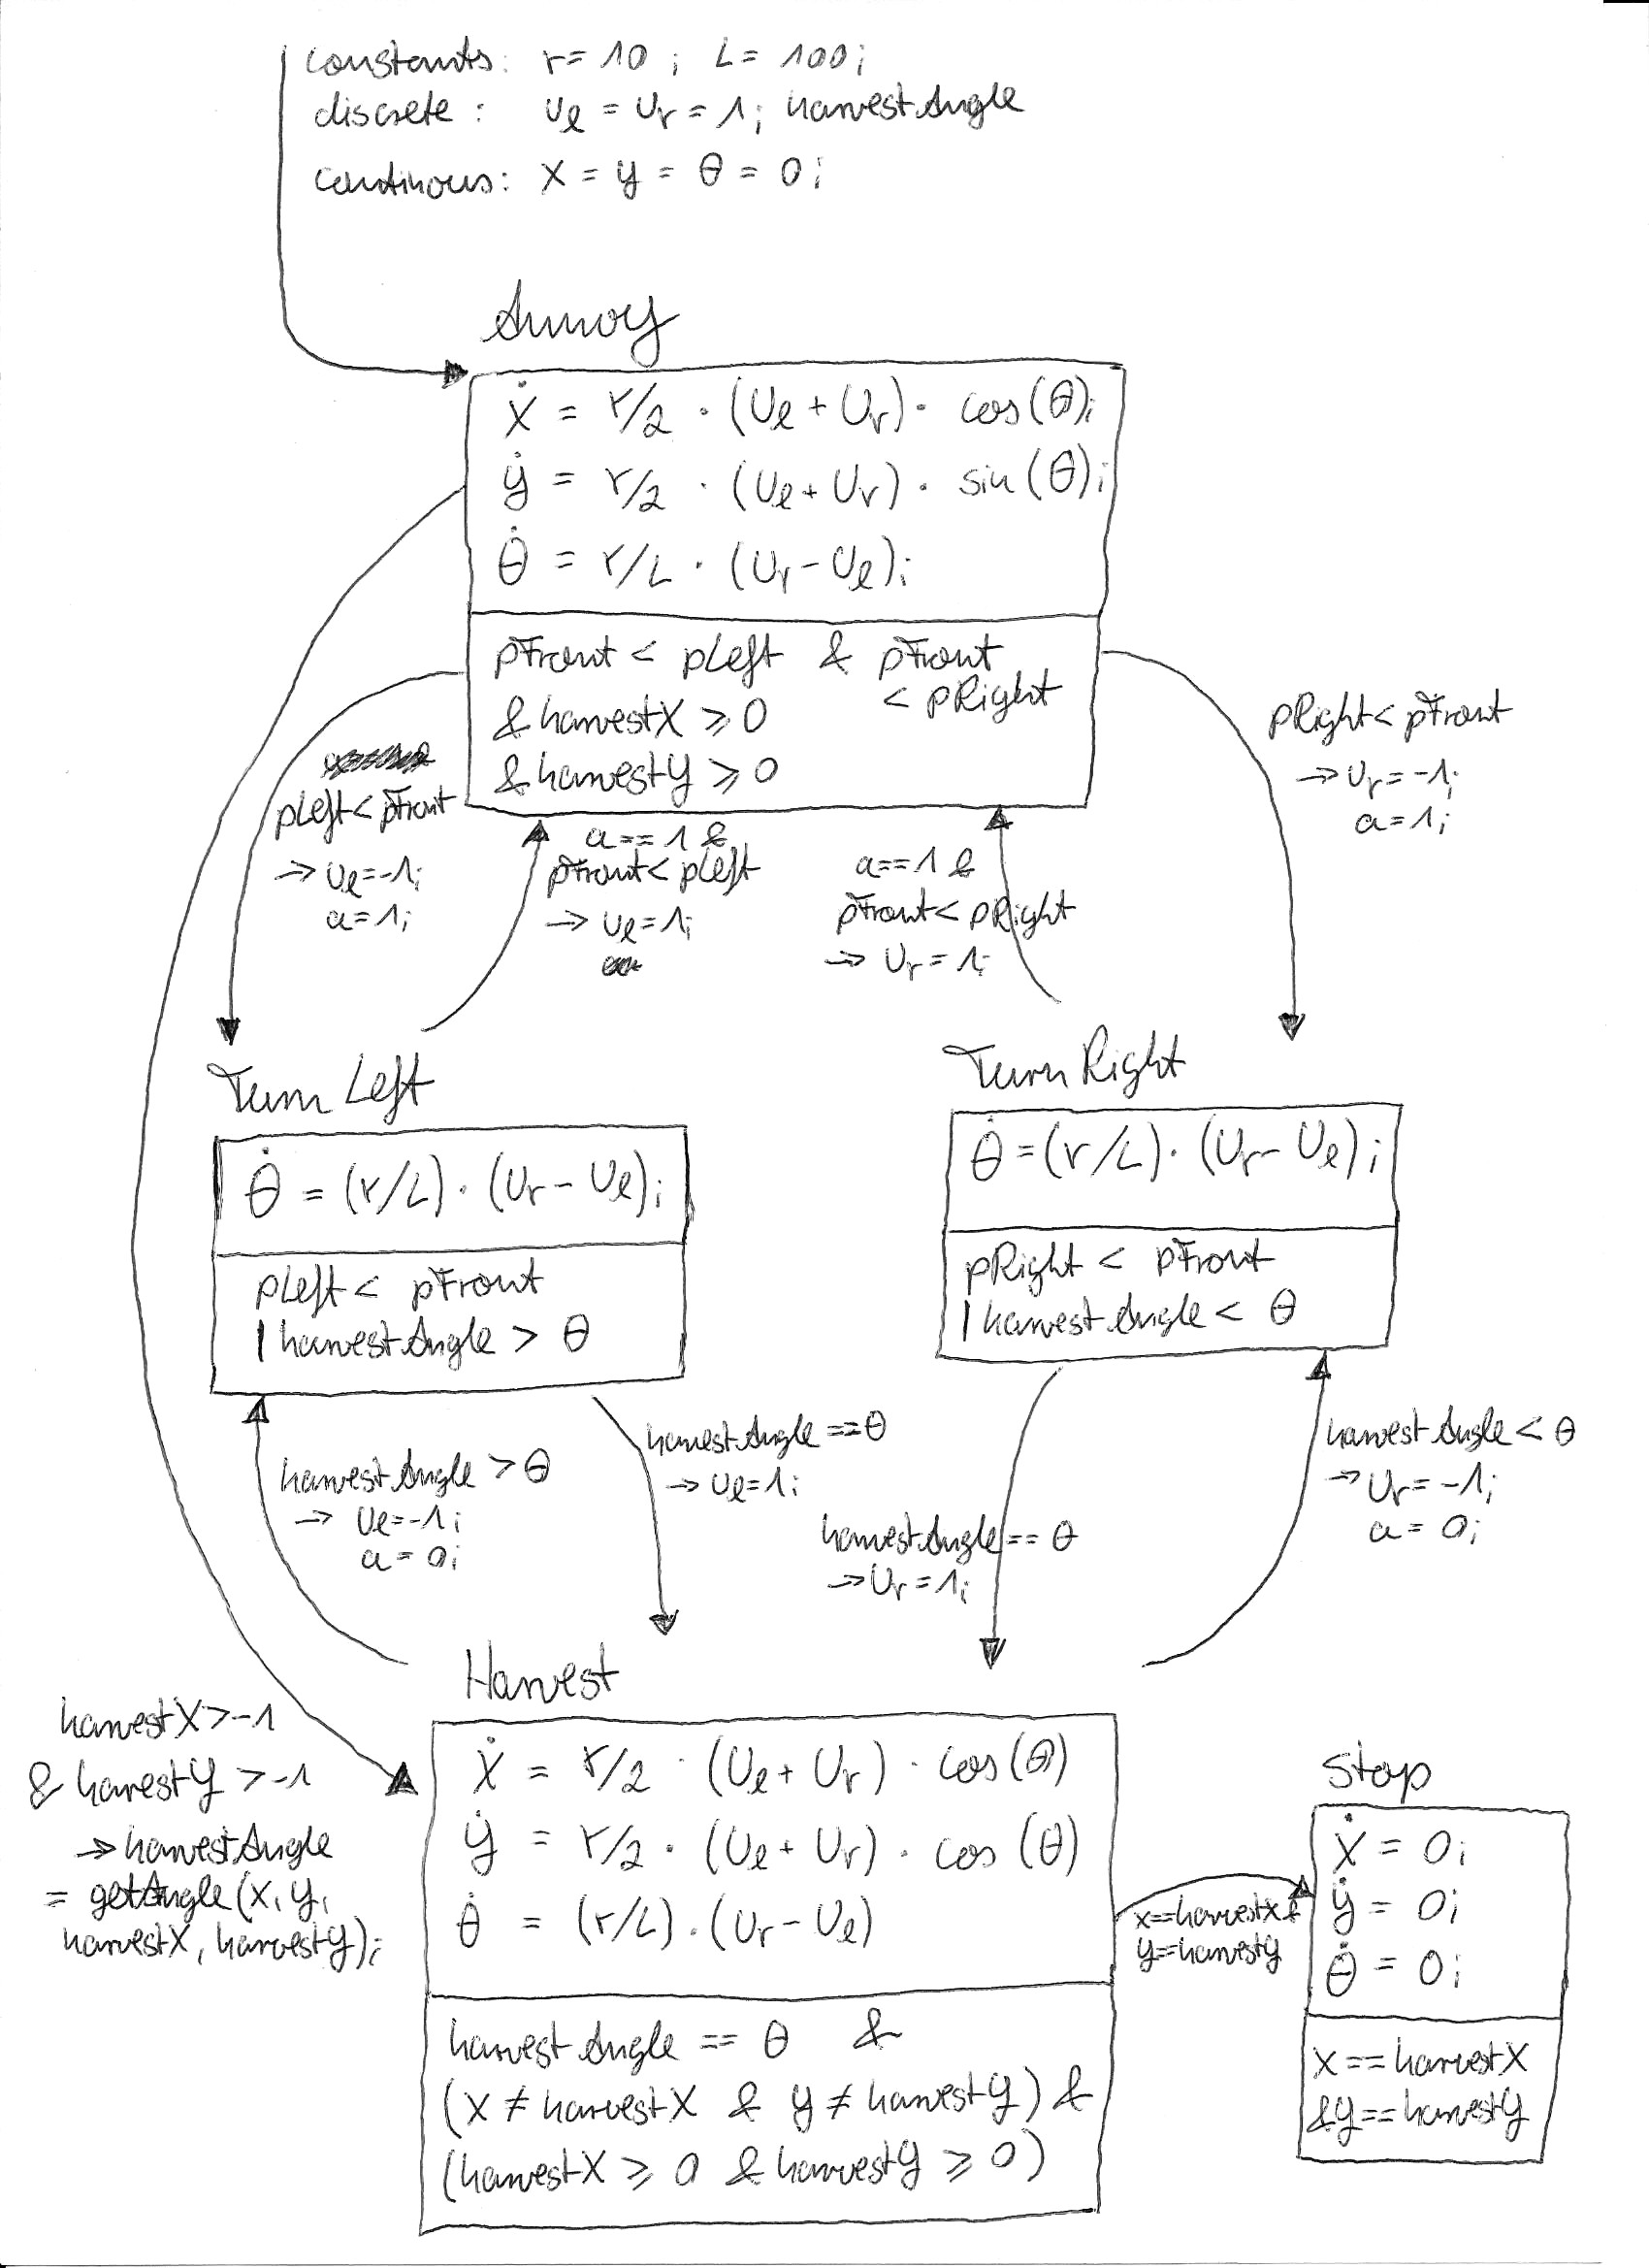
\includegraphics[scale = 0.8]{pictures/hybrid_automata_collector}


\end{document}
